\chapter{Curbe Eliptice} 
\section{Introducere}
\label{sec:sec01}
Folosirea curbelor eliptice in criptografie a fost propusa pentru prima oara in anul 1985 de Victor Miller(IBM) si, independent, de Neal Koblitz. Ideea de baza este folosirea grupului de puncte de pe o curba eliptica in locul grupului $(\mathbb{Z}/p\mathbb{Z})^{*}$. Printre aplicatiile curbelor eliptice se numara constructia criptosistemelor cu chei publice, construirea de generatoare pseudoaleatoare de biti (poate mai cauti ceva aici).
\begin{dfn}
[sursa Guide to elliptic curves menezez]O \textit{curba eliptica} $E$ peste un corp $K$ este definita prin ecuatia:
$$E : y^2 + a_1xy + a_3y = x^3 + a_2x^{2} + a_4x + a_6$$ 
\\unde $a_1, a_2, a_3, a_4, a_5, a_6\in K$, iar discriminantul ecuatiei, $\Delta \neq 0$. Discriminantul ecuatiei este definit astfel:
$$ \begin{cases}
\Delta = -d_2^{2}d_8 - 8d_4^{3} - 27d_6^{2} + 9d_2d_4d_6 \\
d_2 = a_1^{2} + 4a_2 \\
d_4 = 2a_4 + a_1a_3 \\
d_6 = a_3^{2} + 4a_6 \\
d_8 = a_1^{2}a_6 + 4a_2a_6 - a_1a_3a_4 + a_2a_3^{2} - a_4^{2}
\end{cases}$$
\end{dfn}
\begin{dfn}
Fie $L$ orice extensie a corpului $K$. Definim multimea de $L$-puncte rationale peste $E$ astfel: $E(L) = \set {(x, y)\in L\times L: y^2 + a_1xy + a_3y - x^3 - a_2x^{2} - a_4x - a_6 = 0} \cup \set {\infty}$
\end{dfn}
\begin{obs}
In urmatoarele randuri voi face o serie de observatii asupra ecuatiei unei curbe eliptice: \\
(i) Ecuatia de la definitia 2.1 se numeste Ecuatie Weierstrass \\
(ii) Conditia ca discriminantul $\Delta$ sa fie diferit de 0 asigura "netezimea" curbei eliptice, adica nu exista puncte care sa aibe 2 sau mai multe tangente diferite la curba. \\
(iii) L-punctele rationale sunt acele puncte, $(x, y)$ care satisfac ecuatia Weierstrass, cu $x, y \in L$. Punctul de la infinit este considerat un punct L-rational pentru toate extensiile $L$ ale corpului $K$
\end{obs}

\begin{dfn}
Fie $E_1, E_2$ doua curbe eliptice, definite astfel: \\
$E_1 : y^2 + a_1xy + a_3y = x^3 + a_2x^{2} + a_4x + a_6$ \\
$E_2 : y^2 + \overline{a_1}xy + \overline{a_3}y = x^3 + \overline{a_2}x^{2} + \overline{a_4}x + \overline{a_6} $ \\
Spunem ca cele doua curbe sunt \textit{izomorfe} daca exista $u,r,s,t\in K, u\neq 0$ astfel incat schimbarea de variabila $(x, y)\rightarrow (u^2x + r, u^3y + u^2sx + t)$ transforma ecuatia $E_1$ in ecuatia $E_2$. Acest tip de transformare se numeste schimbare "admisibila" de variabila.
\end{dfn}
\begin{dfn}
Ecuatia Weierstrass a unei curbe eliptice poate fi simplificata in mod considerabil, aplicand schimbari admisibile de variabila. Vom trata trei cazuri separate de schimbari de variabila, in functie de caracteristica corpului $K$, ajungand la o forma \textit{simplificata a Ecuatiei Weierstrass.}. Vom aborda trei cazuri, primul fiind $char(K) \neq \set {2,3}$ \\

  1. Fie $K$ un corp si \textit{E} o curba eliptica data prin ecuatia lui Weierstrass. O schimbare admisibila de variabila este:
$(x, y) \rightarrow (\frac{x - 3a_1^{2} - 12a_2}{36}, \frac{y-3a_1x}{216} - \frac{a_1^{3} + 4a_1a_2 - 12a_3}{24})$ \\
Aceasta schimbare transforma ecuatia $E$ in ecuatia 
\begin{center} $y^2 = x^3 + ax + b; a, b\in K$\end{center}
Discriminantul acestei noi ecuatii este $\Delta = -16(4a^3 + 27b^2)$ \\

2. Daca $char(K) = 2$ trebuie sa consideram doua subcazuri. Daca $a_1 \neq 0$, atunci o schimbare admisibila de variabila este: $(x, y) \rightarrow (a_1^2x + \frac{a_3}{a_1}, a_1^3y + \frac{a_1^2a_4 + a_3^2}{a_1^3} )$, care transforma $E$ in:
\begin{center}$y^2 + xy = x^3 + ax^2 + b; a, b\in K$\end{center}
O astfel de ecuatie se numeste \textit{non-supersingulara} si are discriminantul $\Delta = b$ \\
Daca $a_1 = 0$ atunci o schimbare admisibila ar fi $(x, y)\rightarrow (x + a_2, y)$ care transforma curba $E$ in
\begin{center} $y^2 + cy = x^3 + ax + b; a,b,c\in K$ \end{center}
O astfel de ecuatie se numeste \textit{supersingulara} si are discriminantul $\Delta = c^4$
\\

3. Daca $char(K) = 3$ trebuie sa consideram din nou doua subcazuri. Daca $a_1^2 \neq -a_2$ atunci o schimbare admisibila de variabila este
$(x, y) \rightarrow (x + \frac{\alpha}{\beta}, y + a_1x + a_1\frac{\alpha}{\beta} + a_3)$, unde $\alpha = a_4 -a_1a_3$ si $\beta = a_1^2 - a_2$. Ecuatia $E$ devine: 
\begin{center} $y^2 = x^3 + ax^2 + b; a, b\in K$\end{center}
O astfel de ecuatie se numeste \textit{non-supersingulara} si are discriminantul $\Delta = -a^3b$ \\
Daca $a_1^2 = -a_2$ atunci consideram o schimbare admisibila de variabila $(x, y) \rightarrow (x, y + a_1x + a_3)$ care transforma curba $E$ in:
\begin{center} $y^2 = x^3 + ax + b$ \end{center}
O astfel de curba este \textit{supersingulara} si are discriminantul $\Delta = -a^3$
\end{dfn}

\begin{obs}
Vom lucra cu forma simplificata a ecuatiei Weierstrass pe tot parcursul urmatoarelor capitole.
\end{obs}

\subsection{Constructia curbelor eliptice}
\label{subsec:subsec01}

\begin{dfn}
Fie $E$ o curba eliptica peste un corp $K = F_q$. Multimea de puncte $E(F_q)$ impreuna cu operatia de adunare formeaza o structura de grup abelian, cu punctul de la infinit fiind elementul neutru din grup. Acest grup este folosit in criptografia bazata pe curbe eliptice.
\end{dfn}

\begin{dfn}
Numim \textit{ordin} al unei curbe eliptice, numarul de puncte care satisfac ecuatia Weierstrass, cu alte cuvinte cardinalul multimii $E(F_q)$ si il notam cu $\# E(F_q)$. Teorema care urmeaza, datorata lui \textit{Hasse}, ofera o aproximare pentru acest ordin
\end{dfn}
\begin{teo}
Fie $E$ o curba eliptica definita peste $F_q$. Atunci este adevarata relatia:
\begin{center} $q + 1 - 2\sqrt{q}\leq \# E(F_q)\leq q+1 + 2\sqrt{q}$ \end{center}
Intrucat $2\sqrt{q}$ este relativ mic in comparatie cu $q$, putem afirma ca $\# E(F_q) \approx q$
\end{teo}
\begin{teo}
Fie $q = p^m$, unde $p$ este caracteristica corpului $F_q$. Atunci exista o curba eliptica $E$ definita peste acest corp, cu $\# E(F_q) = q+1-t$ ($t$ se numeste urma curbei eliptice $E$) daca si numai daca una dintre urmatoarele conditii este adevarata: \\
(i) $t \not\equiv 0$ mod $p$ si $t^2\leq 4q$ \\
(ii) m este impar si $t=0$ sau $t^2 = 2q$ si $p=2$ sau $t^2 = 3q$ si $p=3$ \\ 
(iii) m este par si $t^2 = 4q$ sau $t^2 = q$ si $p\not\equiv 1$ mod $3$ sau $t= 0$ si $p\not\equiv 1$ mod $4$
\end{teo}
\begin{dfn}
Fie $p$ caracteristica corpului $F_q$. Numim curba eliptica \textit{supersingulara}, daca $p$ divide $t$, unde t este urma curbei. Altfel, curba $E$ este \textit{non-supersingulara}
\end{dfn}
\begin{teo}
Fie $E$ o curba eliptica peste corpul $F_q$ si fie ordinul acesteia $\# E(F_q)= q+ 1-t$. Atunci, $\# E(F_q) = q+ 1 - V_n$, unde definim sirul $\set {V_n}$ recursiv prin formula $V_0 = 2, V_1=t$ si $V_n = V_1V_{n-1} - qV_{n-2}, \forall n\geq 2$
\end{teo}
Urmatoarea teorema descrie structura grupului pentru o curba eliptica. Vom nota un grup ciclic de ordin n, cu $Z_n$.
\begin{teo}
Fie E o curba eliptica definita peste $F_q$. Atunci grupul $E(F_q)$ este izomorfic cu $Z_{n_1} \oplus Z_{n_2}$, unde $n_1, n_2\in Z$, unici determinati, cu $n_2$ care divide atat $n_1$ cat si $q-1$. Daca $n_2=1$, spunem ca $E(F_q)$ este grup ciclic.
\end{teo}

\subsection{Reprezentari ale punctelor de pe o curba eliptica}
\label{subsec:subsec02}
De multe ori, in efectuarea operatiile pe curbe eliptice, poate fi avantajos sa reprezentam un punct in alte coordonate decat cele afine(sectiunea 2.3.1). De exemplu, in calculul sumei a doua puncte(operatie care la randul ei este folosita in algoritmii pentru inmultirea cu un scalar si in inmultirea multipla) se observa necesitatea de a efectua operatia de invers modular de mai multe ori. Acesta operatie este costisitoare din punct de vedere computational, astfel vom folosi diferite tipuri de reprezentari.
\begin{dfn}
Fie $K$ un corp si $c, d\in \mathbb{N}$. Definim o relatie de echivalenta peste multimea $K^3\setminus \set {(0, 0, 0)}$ ca fiind :
\begin{center} $(X_1, Y_1, Z_1) \equiv (X_2, Y_2, Z_2)$ daca $X_1 = \lambda ^cX_2, Y_1 = \lambda ^d Y_2, Z_1 = \lambda Z_2, \lambda\in K^{*}$\end{center}
Exista o corespondenta $1-1$ intre multimea de puncte in coordonate proiective $P(K)^{*} = \set {(X, Y, Z): X, Y, Z\in K, Z\neq 0}$ si multimea punctelor in coordonate afine, $A(K) = \set {(x, y): x, y\in K}$
\end{dfn}
\begin{dfn}
Consideram $c=1, d=1$ in definitia \textit{coordonatelor proiective}. Acestea se numesc \textit{coordonate proiective standard}. Punctu l in coordonate proiective $(X, Y, Z), Z\neq 0$ corespunde punctului in coordonate afine $(X/Z, Y/Z)$. Ecuatia curbei eliptice devine:
\begin{center}  $Y^2Z = X^3 + aXZ^2 + bZ^3$ \end{center}
Punctul de la infinit este $(0, 1, 0)$ in timp ce inversul unui punct oarecare este $(X, -Y, Z)$
\end{dfn}
\begin{dfn}
Consideram $c=2, d=3$. Acest sistem de coordonate se numesc coordonate \textit{proiective Jacobi}. Punctul $(X, Y, Z), Z\neq 0$ corespunde punctului 
in coordonate afine $(X/Z^2, Y/Z^3)$. Ecuatia curbei devine:
\begin{center} $Y^2 = X^3 + aXZ^4 + bZ^6$ \end{center}
Punctul de la infinit este $(1, 1, 0)$, iar inversul unui punct este $(X, -Y, Z)$
\end{dfn}
\begin{dfn}
\textit{Coordonatele Chudnovsky} sunt obtinute din coordonatele Jacobi, adaugand niste reduntante. Astfel, un punct reprezentat in acest tip de coordonate, arata in acest fel : $(X, Y, Z, Z^2, Z^3)$. Acest tip de reprezentare aduce imbunatatiri de performanta cand folosim anumiti algoritmi specializati pentru inmultirea cu un scalar.
\end{dfn}

\begin{obs}
Se poate folosi $Z = 1$ in implementari pentru a simplifica calculele.
\end{obs}

\section{Aritmetica curbelor eliptice}
\label{sec:sec02}
In aceasta sectiune vom prezenta operatiile din corpul finit format de punctele de pe o curba eliptica(adunarea,  inmultirea cu un scalar) precum si operatia de inmultire multipla cu scalari. La inceput vom oferi o privire de ansamblu asupra acestor operatii, oferind definitii, apoi vom intra in delalii in sectiunea 2.3, oferind inclusiv implementarea unor algoritmi eficienti pentru aceste operatii.

\begin{dfn}
Adunarea a doua puncte de pe o curba eliptica este foarte intuitiva din punct de vedere geometric. Fie $P, Q$ doua puncte si $R$ suma lor. Rezultatul este obtinut astfel. Mai intai desenam o linie intre $P, Q$. Acesta linie intersecteaza curba intr-ul al treilea punct. Punctul $R$ este reflectia la axa $Ox$ a acestui punct(Figura 2.1a). Dublul unui punct $P(2P = R)$ este definit astfel. Desenam o tangenta la curba eliptica in P, aceasta intersectand curba intr-un punct secundar. Punctul $R$ este din nou reflexia la axa $Ox$(Figura 2.1b).  
\end{dfn}

\begin{obs}
Formulele algebrice pentru adunarea a doua puncte difera in functie de sistemul de coordnate folosit, sau tipul de corp algebric peste care este definita curba eliptica(corp prim, binar sau de extensie).
\end{obs}

\begin{figure}[htp]
\centering
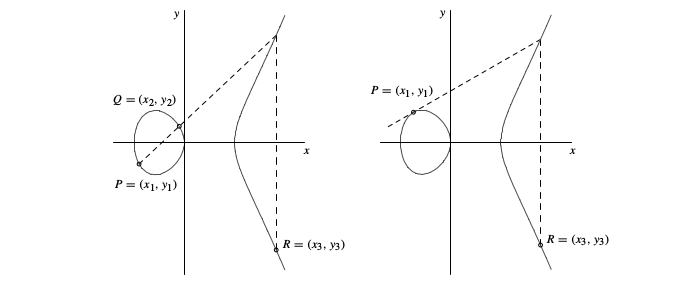
\includegraphics[width=13cm]{chapters/Addition.png}
\caption{Adunarea si dublarea unui punct pe o curba eliptica}
\label{fig:lion}
\end{figure}

\begin{dfn}
O alta operatie fundamentala este cea a inmultirii unui punct $P$ de pe o curba eliptica, cu un scalar, $k\in \mathbb{Z}$. Exista multe metode de a face acest lucru, de la metoda brute force de a face k adunari repetate pana la metode mai rafinate, precum cea a ferestrei glisante, care inbunatatesc considerabil performanta operatiei. Vom discuta in sectiunile care urmeaza algoritmi eficienti de inmultire. 
\end{dfn}

\begin{dfn}
O operatie asemanatoare celei de inmultire cu un scalar, este cea de inmultire multipla cu scalari. Fie doua puncte, $P, Q$ de pe o curba eliptica si doi scalari, $k, l\in \mathbb{Z}$. Dorim sa aflam rezultatul $kP + lQ$. Evident, precum la operatia de inmultire cu un scalar putem aplica o metoda directa, de a inmulti punctul $P$ cu scalarul $k$ respectiv punctul $Q$ cu scalarul $l$ si apoi facem o adunare de puncte. Acest lucru este insa ineficient, intrucat exista si aici metode mai rapide de a calcula acest lucru. Aceasta operatie de inmultire rapida este una extrem de folosita in criptografia pe curbe eliptice, aparand de exemplu, in cadrul unor protocoale criptografice, precum ECDSA, iar implementarea ineficienta e acesteia duce la mari probleme de performanta. 
\end{dfn}

\begin{obs}
Operatia de adunare pe o curba eliptica este corespondenta operatiei de inmultire
in sistemele cu chei publice obisnuite, iar adunarea multipla este corespondenta
exponentierii modulare din acestea.
Desi regulile de calcul in grupul punctelor unei curbe eliptice par destul de complicate, aritmetica acestora poate fi implementata extrem de eflcient, calculele in acest grup fiind realizate mult mai rapid decat cele din grupul $Z_p$, deoarece operatia de invers este una necostisitoare din punct de vedere computational.
\end{obs}

\section{Studiu Comparativ}
\label{sec:sec03}
In aceasta subsectiune vom aborda cele trei operatii de baza, adunarea, inmultirea cu un scalar si inmultirea multipla, prezentand la fiecare sectiune o analiza a eficientei metodei alese. Implementarea eficienta si corecta a acestor operatii reprezinta un prim pas foarte important spre dezvoltarea unor criptosisteme bazate pe curbe eliptice.
\\ Pentru implementare am ales limbajul de programare Python, versiunea 3.5.2, iar hardware-ul folosit in tabelele de test este: Quad Core CPU, i7-4700HQ, 2.4 GHz, 64 bit OS, 16 GB RAM.

\subsubsection{Arhitectura aplicatiei}
\label{sec:sec01}
arhitectura(Inclusiv grupul folosit, curbele eliptice Nist), diagrama UML cu clasele

\begin{figure}[htp]
\centering
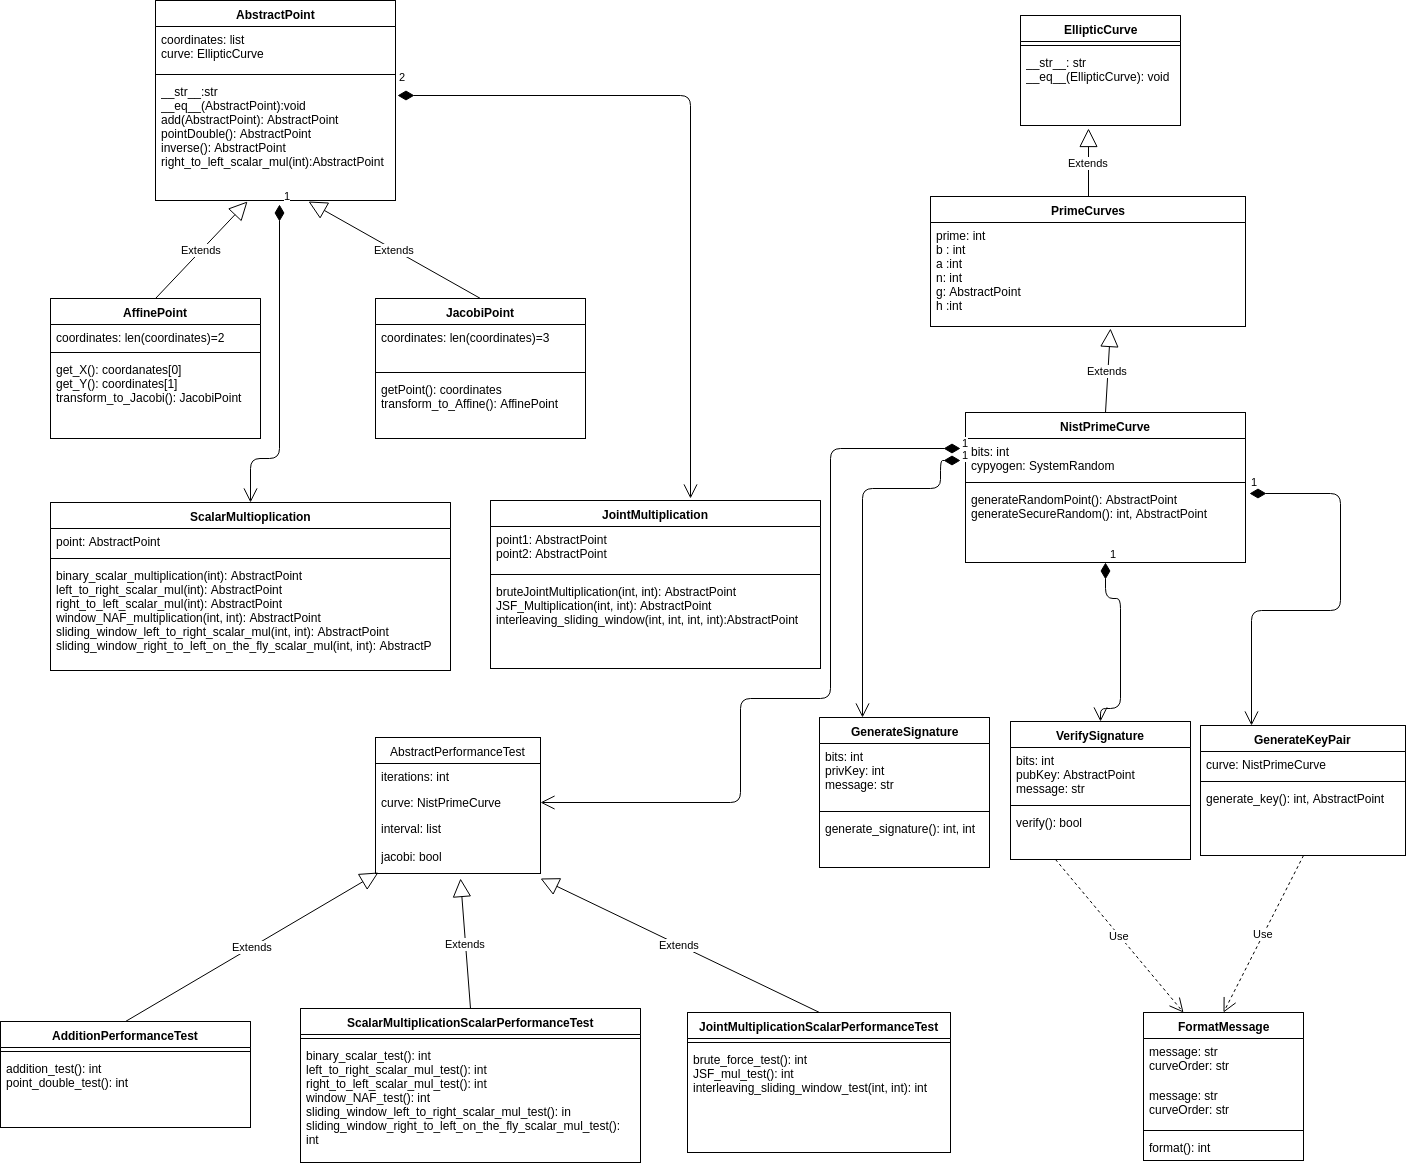
\includegraphics[width=17.5cm]{chapters/Arhitectura.png}
\caption{Arhitectura Aplicatiei}
\label{fig:lion}
\end{figure}

\subsection{Adunarea punctelor de pe o curba eliptica}
\label{subsec:subsec02}
In aplicatie am implementat operatia de adunare pentru coordonate Afine si pentru coordonate Jacobiene. Vom oferi formulele de calcul pentru cele tipuri de adunare si apoi vom compara eficienta celor doua implementari.
\begin{dfn}
Pentru puncte reprezentate prin coordonate afine formulele de calcul sunt dupa cum urmeaza.Fie doua puncte, $P(x_{1}, y_1), Q(x_2, y_2)\in E(F_p)$. Notam cu $R(x_3, y_3) = P + Q$. Formulele pentru adunarea a doua puncte pot fi demonstrate matematic destul de usor, pornind de la ideea ca $P, Q$ si simetricul rezultatului fata de axa $Ox$ se afla pe aceasi dreapta, respectiv pe aceasi curba eliptica.

$\begin{cases} 
    x_3 = \lambda^2 - x_1 - x_2 \\
    y_3 =  \lambda (x_1-x_3) - y_1
   \end{cases}$
 \\cu 
 \\$
 \lambda = 
 \begin{cases}
 \frac{y_2 - y_1}{x_2 - x_1}, P \neq Q \\ 
 \frac{3x^{2}_1 + a}{2y_1}, P = Q
 \end{cases}$ \\
\end{dfn}

\begin{dem}
Fie $P(x_1, y_1), Q(x_2, y_2)\in E(F_p)$ Punctele se afla pe aceasi dreapta. Scriind ecuatia dreptei care trece prin cele doua puncte si considerand ca $-R\in E(F_p)$, rezolvam sistemul de ecuatii:
$\begin{cases} 
    0 = \begin{vmatrix}
			x_1 & y_1 & 1 \\ 
			x_2 & y_2 & 1 \\ 
			x & y & 1  \\ 
			\end{vmatrix} \\
    y^2 =  x^3 + ax + b
   \end{cases}$
   Panta dreptei este $\lambda = \begin{cases}
 \frac{y_2 - y_1}{x_2 - x_1}, P \neq Q \\ 
 \frac{3x^{2}_1 + a}{2y_1}, P = Q
 \end{cases}$
 \\Inlocuind in formula curbei eliptice obtinem formulele din definita precedenta.
\end{dem}

Operatiile de adunare si dublare a unui punct de pe o curba eliptica sunt operatii care au o importanta deosebita intrucat sunt folosite in fiecare algoritm de la sectiunile urmatoare(inmultire cu un scalar si inmultire multipla).
\\ In coordonate afine algoritmul de adunare este clar, algoritmul fiind o simpla aplicare a formulelor de mai sus. Operatia cea mai costisitoare din algoritmul de mai jos e cea de invers modular(in calculul lui $\lambda$). Aceasta operatie se face cu ajutorul algoritmului lui Euclid Extins.

\begin{lstlisting} 
def add(self, other):
	if self is None:
		return other
	if other is None:
		return self

	if self == other:
		_lambda = ((3 * self.x ** 2 + self.elliptic_curve.a) 
                   * inv(2 * self.y,self.elliptic_curve.prime)) % 
                   self.elliptic_curve.prime
	else:
		_lambda = ((other.y - self.y) * 
                  inv(other.x - self.x, self.elliptic_curve.prime)) %
                  self.elliptic_curve.prime
	x3 = (_lambda ** 2 - self.x - other.x) % self.elliptic_curve.prime
	y3 = (_lambda * (self.x - x3) - self.y) % self.elliptic_curve.prime
	return Point(self.elliptic_curve, [x3, y3])
\end{lstlisting}

Ideea de la urmatorii doi algoritmi  este sa folosim un set de coordonate redundante(coordonate Jacobiene) pentru a evita calculul inversului modular.

\begin{lstlisting}
def add(self, other):
    if self is None:
        return other
    if other is None:
        return self

    u1 = (self.x * other.z ** 2) % self.curve.prime
    u2 = (other.x * self.z ** 2) % self.curve.prime
    s1 = (self.y * other.z ** 3) % self.curve.prime
    s2 = (other.y * self.z ** 3) % self.curve.prime
    if u1 == u2:
        if s1 != s2:
            return None
        else:
            return self.point_double()

    h = (u2 - u1) % self.curve.prime
    r = (s2 - s1) % self.curve.prime
    x3 = (r ** 2 - h ** 3 - 2 * u1 * h ** 2) % self.curve.prime
    y3 = (r * (u1 * h ** 2 - x3) - s1 * h ** 3) % self.curve.prime
    z3 = (h * self.z * other.z) % self.curve.prime
    return Jacobi_Point([x3, y3, z3, pow(z3, 2, self.curve.prime), 
           pow(z3, 3, self.curve.prime)], self.curve)
\end{lstlisting}

\begin{lstlisting}
def point_double(self):
    if self is None:
        return None
    if self.y == 0:
        return None
    s = (4 * self.x * self.y ** 2) % self.curve.prime
    m = (3 * self.x ** 2 + self.curve.a * self.z ** 4) % self.curve.prime
    _x = (m ** 2 - 2 * s) % self.curve.prime
    _y = (m * (s - _x) - 8 * self.y ** 4) % self.curve.prime
    _z = (2 * self.y * self.z) % self.curve.prime
    return Jacobi_Point([_x, _y, _z, pow(_z, 2, self.curve.prime), 
	   pow(_z, 3, self.curve.prime)], self.curve)
\end{lstlisting}

In continuare, vom face o comparatie intre cele doua metode de adunare, cea cu coordonate afine si cea in coordonate Jacobiene. In teste am am generat random doua numere pe o curba eliptica si le-am adunat. Am cronometrat 1000 de iteratii la fiecare test. Se poate observa per total ca adunarea in coordonate Jacobiene este de doua ori mai rapida decat cea in coordonate afine.

\begin{tabular}{ |p{3cm}||p{3cm}|p{3cm}|p{3cm}|  }
 \hline
 \multicolumn{4}{|c|}{Adunarea punctelor de pe curbe eliptice} \\
 \hline
 Curba NIST& Coordonate &Metoda &Timp de executie(secunde)\\
 \hline
 P192   & Afine    &Adunare& 5.22\\
 P192&Afine  & Dublare & 5.19\\
 P192 &Jacobiene & Adunare& 2.6\\
 P192&Jacobiene & Dublare & 2.61\\
 P224& Afine & Adunare & 6.66\\
 P224& Jacobiene & Adunare   &3.32\\
 P256& Afine  & Adunare& 8.47\\
 P256& Jacobiene  & Adunare& 4.52\\
 P384& Afine  & Adunare& 18.06\\
 P384& Jacobiene  & Adunare& 8.96\\
 \hline
\end{tabular}

\subsection{Inmultirea cu un scalar}
\label{subsec:subsec03}


Putem aborda metoda problema multiplicarii cu un scalar in diferite feluri, de la cele mai ineficiente metode(apelararea functiei de adunare de cate ori este nevoie) pana la metode sofisticate si eficiente, cum ar fi inmultirea cu fereastra glisanta.

\subsubsection{Metoda Binara}

Prima metoda pe care am implementat-o este cea binara. Algoritmul consta in procesarea binara a scalarului de la cel mai nesimnificativ bit la cel mai semnificativ(de la dreapta la stanga deci). Exista si o varianta a algoritmului de la stanga la dreapta, echivalenta. Ideea este adaugam la resultat punctul P(cel care dorim sa il inmultim cu yn scalar) de fiecare data cand avem punctul P si sa dublam P-ul dupa fiecare bit parcurs.

\begin{lstlisting}
def binary_scalar_multiplication(self, d):
    P = self.point
    if d == 0:
        return None  # returnam punctul de la "infinit" daca d este 0
    if d == 1:
        return P
    result = None
    while d > 0:
        if d % 2:
            result = P.add(result)
        d //= 2
        P = P.add(P)
    return result
\end{lstlisting}

\subsubsection{Reprezentari cu semn}

Un avantaj major al curbelor eliptice, este faptul ca in grupul format de punctele de pe o astfel de curba, operatia de invers este foarte eficienta. Astfel, daca consideram 2 puncte $P, Q$ intr-un astfel de grup, putem calcula $P + Q$ si $P - Q$ cu acelasi cost computational. Aceasta observatie este foarte importanta in eficientizarea algoritmilor de inmultire cu un scalar. Calculul inversului avand un cost neglijabil din punct de vedere computational, nu este necesar sa ne limitam la $\set{0, 1}$ in reprezentarea unui scalar. Introducem astfel conceptul de reprezentare cu semn.

\begin{dfn}
[Sursa: Solinas] Fie $n\in\mathbb{N}$. O reprezentare a lui cu semn poate fi notata astfel: $n = <u_{l-1}u_{l-2}...u_1u_0>$, unde $u_i\in\set{0, -1, 1}$. Astfel $n = \sum_{i=0}^{l-1} u_i 2^{i}$. Exista o infinitate de astfel de reprezentari.
\end{dfn}
\begin{dfn}
Reprezentarea cu semn optima pentru operatia de inmultire cu un scalar este asa numita NAF, sau Non Adjacent Form. Aceasta are proprietatea ca nu exista doua elemente consecutive din reprezentarea cu semn diferite de 0.
\end{dfn}

\begin{teo}
NAF-ul are urmatoarele proprietati:
\begin{itemize}
  \item Orice numar natural are un NAF
  \item NAF-ul unui numar este unic
  \item Lungimea NAF-ului unui numar natural este cu cel mult o unitate mai mare decat expansiunea binara a numarului 
  \item NAF-ul are distanta Hamming minima dintre toate reprezentarile cu semn
\end{itemize}
\end{teo}

In continuare voi prezenta un algoritm eficient pentru calculul reprezentarii NAF.

\begin{lstlisting}
def naf(d):
    i = 0
    res = []
    while d >= 1:
        if d % 2 == 0:
            res.append(0)
        else:
            res.append(2 - d % 4)
            d -= res[i]
        d //= 2
        i += 1
    return res[::-1]
\end{lstlisting}

Avand la dispozitie metoda pentru aflarea reprezentarii cu semn a unui numar natural, putem eficientiza metoda binara. Algoritmul de la stanga la dreapta pentru calculul lui $dP$, unde d este scalarul si $P$ este un punct de pe o curba eliptica, apeleaza functia pentru reprezentare cu semn. Parcurgem aceasta reprezentare si la fiecare bit de 0 dublam rezultatul, la bitul de 1 adunam punctul $P$ sa la bitul $-1$ scadem $P$.

\begin{lstlisting}
def left_to_right_scalar_mul(self, d):
    signed_d = naf(d)
    result = None
    for i in signed_d:
        if result is None:
            result = None
        else:
            result = result.point_double()
        if i == 1:
            result = self.point.add(result)
        if i == -1:
            result = self.point.inverse().add(result)
    return result
\end{lstlisting}

Algoritmul de la dreapta la stanga functioneaza in acelasi mod, singura diferenta fiind faptul ca NAF-ul este calculat in aceasi bucla while in care calculam rezultatul final. In acea bucla descompunem scalarul, tinem bit-ul curent intr-o variabila si in functie de valoarea acestuia modificam rezultatul. 

\begin{lstlisting}
def right_to_left_scalar_mul(self, d):
    result = None
    R = self.point
    while d >= 1:
        if d % 2 == 1:
            u = 2 - (d % 4)
            d -= u
            if u == 1:
                result = R.add(result)
            else:
                result = R.inverse().add(result)
        d //= 2
        R = R.point_double()
    return result
\end{lstlisting}

\subsubsection{Metoda cu fereastra}
Algoritmii care se folososesc de reprezentarea cu semn a scalarului pot fi inbunatatiti daca avem disponibila mai multa memorie. Vom procesa $w$ cifre din scalar la o iteratie, unde $w$ reprezinta latimea ferestrei.

\begin{dfn}
Fie $w\geq 2$ un numar natural. Numim o reprezentare NAF de latime $w$ pentru un scalar $n\in\mathbb{N}$, notata cu $w-NAF$, un sir de numere $n = <u_{l-1}u_{l-2}...u_1u_0>$ astfel incat $|u_i| < 2^{w-1}$ si $n = \sum_{0}^{l-1}u_i2^i$ astfel incat cel mult una din $w$ cifre consecutive din sir este diferita de 0.
\end{dfn}

Un algoritm eficient pentru calculul $w-NAF$ va fi prezentat in continuare. Functia mods este modulo cu semn, adica pentru un scalar $d$, avem $d$ mods $2^w=u$, unde u este un numar intreg care satisface $u\equiv d$ mod $2^w$ si $-2^{w-1}\leq u\leq 2^{w-1}$.

\begin{lstlisting}
def w_NAF(d, w):
    i = 0
    res = []
    while d >= 1:
        if d % 2 == 0:
            res.append(0)
        else:
            res.append(mods(d, w))
            d -= res[i]
        d //= 2
        i += 1
    return res[::-1]
\end{lstlisting}

Metoda cu fereseatra reprezinta o generalizare a algoritmului de inmultire precedent, aducand un plus de performanta prin scaderea numarului de adunari necesare in calculul multiplului unui punct oarecare $P$ de pe o curba eliptica. Aici vom folosi $w-NAF$ in loc de $NAF$. In algoritm vom precalcula si stoca valorile pentru $iP$ si $i\in\set{1, 2^{w-1}}$. Astfel cand parcurgem $w-NAF$ -ul numarului in functie de cifra gasita vom aduna sau scadea din rezultat valoarile potrivite din multimea de valori precalculate.

\begin{lstlisting}
def window_NAF_multiplication(self, d, w):
    d = w_NAF(d, w)
    _P = {}
    for i in range(1, 2**(w-1), 2):
        _P[i] = self.right_to_left_scalar_mul(i)
    Q = None
    for i in range(0, len(d)):
        if Q is None:
            Q = None
        else:
            Q = Q.point_double()
        if d[i] != 0:
            if d[i] > 0:
                Q = _P[d[i]].add(Q)
            else:
                Q = _P[-d[i]].inverse().add(Q)
    return Q
\end{lstlisting}

\subsubsection{Metoda cu fereastra glisanta}
Pentru a eficientiza metoda cu fereastra fixa prezentata mai sus, vom procesa folosi o asa zisa "fereastra glisanta" asupra cifrelor din $w-NAF$ cu scopul de a face un compromis intre numarul de adunari si dublari. Primul algoritm apeleaza functia pt $w-NAF$ si gliseaza o fereastra de latime $w$ peste reprezentare cu semn a scalarului astfel incat valoarea in fereastra sa fie impara(pentru a reduce numarul de precalculari). Idea de la al doilea algoritm este sa calculam $w-NAF$ in aceasi bucla in care facem calculul propiu zis al multiplicarii.

\begin{lstlisting}
def sliding_window_right_to_left_scalar_mul(self, d, w):
    d = w_NAF(d, w)
    Q = None
    i = 0
    m = 2 * ((2 ** w - (-1)**w) // 3) - 1
    _P = {}
    for _i in range(1, m + 1, 2):
        _P[_i] = self.left_to_right_scalar_mul(_i)
    while i < len(d):
        if d[i] == 0:
            if Q is None:
                Q = None
            else:
                Q = Q.point_double()
            i += 1
        else:
            s = max(len(d) - i - w + 1, 0)
            s = len(d) - 1 - s
            while d[s] == 0:
                s -= 1
            u = NAF(d[i:s + 1])
            for j in range(1, i - s + 2):
                if Q is not None:
                    Q = Q.point_double()
                else:
                    Q = None
            if u > 0:
                Q = _P[u].add(Q)
            if u < 0:
                Q = Q.add(_P[-u].inverse())
            i = 1 + s
    return Q
\end{lstlisting}

\begin{lstlisting}
def sliding_window_right_to_left_on_the_fly_scalar_mul(self, k, w):
    R = self.point
    m = 2**(w-1) - 1
    Q = {}
    for i in range(1, m + 1, 2):
        Q[i] = None
    while k >= 1:
        if k % 2 == 1:
            t = mods(k, w)
            if t > 0:
                Q[t] = R.add(Q[t])
            if t < 0:
                Q[-t] = R.inverse().add(Q[-t])
            k -= t
        R = R.point_double()
        k //= 2
    for i in range(3, m + 1, 2):
        if Q[i] is not None:
            Q[1] = Q[i].right_to_left_scalar_mul(i).add(Q[1])
    return Q[1]
\end{lstlisting}

Pentru teste am decis sa aleg diferite intervale pentru marimea scalarului. Pentru fiecare test sunt rulate 1000 de iteratii cu scalari alesi random in intervalul $5-32$ biti respectiv $128-198$ si $300-384$ pentru curbele $P192$ si respectiv $P384$. Se observa eficienta metodelor cu fereastra pentru numere mari, algoritmul de inmultire care foloseste reprezentarea cu semn fiind foarte eficient pentru numere mici. De asemenea nu se observa o inbunatatirea a eficientei algoritmilor daca procesam de la stanga la dreapta sau de la dreapta la stanga sau la fereastra glisanta, cand facem calculul $w-NAF$-ului in aceasi bucla while in care calculam rezultatul.

Pentru scalari mari, cele mai bune rezultate au fost obtinute cu o fereastra glisanta de latime 4, algoritmul pierzand din eficienta pentru ferestre de latime mai mare din cauza costului mare din punct de vedere computational al precalculului. 

De asemenea putem observa beneficiul impresionant adus de folosirea coordonatelor Jacobiene, acestea aducand inbunatatiri consistente de performanta, algoritmii fiind de aproximativ cinci ori mai rapizi in aceste coordonate. 


\begin{tabular}{ |p{5cm}||p{3cm}|p{3cm}|p{2cm}|p{1cm}|  }
 \hline
 \multicolumn{5}{|c|}{Curba P192} \\
 \hline
 Algortitm& Coordonate &Intervalul &Fereastra &Timp\\
 \hline
 Alg Binar & Afine  &$[2^{5},2^{32}]$& - & 2.48\\
 Alg Binar&Jacobiene  & $[2^{5},2^{32}]$ & - & 0.6\\
 Alg Binar&Jacobiene  & $[2^{128},2^{192}]$ & - & 3.88\\
 Inmultire de st. la dr. & Jacobian & $[2^{5},2^{32}]$& - & 0.39\\
 Inmultire de st. la dr. & Afine & $[2^{128},2^{192}]$& - & 14.04\\
 Inmultire de st. la dr. & Jacobian & $[2^{128},2^{192}]$& - & 2.49\\
 Inmultire de dr. la st. &Afine & $[2^{128},2^{192}]$ & - & 14.33\\
 Inmultire de dr. la st. &Jacobiene & $[2^{5},2^{32}]$ & - & 0.41\\
 Inmultire de dr. la st. &Jacobiene & $[2^{128},2^{192}]$ & - & 2.52\\
 Metoda cu fereastra& Jacobiene & $[2^{5},2^{32}]$ & 3 & 0.42\\
 Metoda cu fereastra& Jacobiene & $[2^{128},2^{192}]$ & 3 & 2.38\\
 Metoda cu fereastra& Jacobiene & $[2^{128},2^{192}]$ & 4 & 2.32\\
 Fereastra glisanta st. la dr.& Jacobiene  & $[2^{5},2^{32}]$& 3 & 0.51\\
 Fereastra glisanta st. la dr.& Jacobiene  & $[2^{128},2^{192}]$& 3 & 2.68\\
  Fereastra glisanta st. la dr.& Jacobiene  & $[2^{128},2^{192}]$& 4 & 2.04\\
 Fereastra glisanta dr. la st.& Jacobiene  & $[2^{128},2^{192}]$& 3 & 2.47\\
 Fereastra glisanta dr. la st.& Jacobiene  & $[2^{128},2^{192}]$& 4 & 2.41\\
 Fereastra glisanta dr. la st.& Jacobiene  & $[2^{128},2^{192}]$& 5 & 2.58\\
 \hline
\end{tabular}

\begin{tabular}{ |p{5cm}||p{3cm}|p{3cm}|p{2cm}|p{1cm}|  }
 \hline
 \multicolumn{5}{|c|}{Curba P384} \\
 \hline
 Algortitm& Coordonate &Intervalul &Fereastra &Timp\\
 \hline
 Alg Binar & Afine  &$[2^{5},2^{32}]$& - & 5.5\\
 Alg Binar&Jacobiene  & $[2^{5},2^{32}]$ & - & 1.12\\
 Alg Binar&Jacobiene  & $[2^{300},2^{384}]$ & - & 13.98\\
 Inmultire de st. la dr. & Jacobian & $[2^{5},2^{32}]$& - & 0.66\\
 Inmultire de st. la dr. & Afine & $[2^{300},2^{384}]$& - & 59.62\\
 Inmultire de st. la dr. & Jacobian & $[2^{128},2^{192}]$& - & 8.33\\
 Inmultire de dr. la st. &Afine & $[2^{300},2^{384}]$ & - & 59.58\\
 Inmultire de dr. la st. &Jacobiene & $[2^{5},2^{32}]$ & - & 0.69\\
 Inmultire de dr. la st. &Jacobiene & $[2^{300},2^{384}]$ & - & 8.69\\
 Metoda cu fereastra& Jacobiene & $[2^{5},2^{32}]$ & 3 & 0.68\\
 Metoda cu fereastra& Jacobiene & $[2^{300},2^{384}]$ & 3 & 8.2\\
 Metoda cu fereastra& Jacobiene & $[2^{300},2^{384}]$ & 4 & 7.89\\
 Fereastra glisanta st. la dr.& Jacobiene  & $[2^{5},2^{32}]$& 3 & 0.85\\
 Fereastra glisanta st. la dr.& Jacobiene  & $[2^{300},2^{384}]$& 3 & 8.73\\
  Fereastra glisanta st. la dr.& Jacobiene  & $[2^{300},2^{384}]$& 4 & 6.46\\
 Fereastra glisanta dr. la st.& Jacobiene  & $[2^{300},2^{384}]$& 3 & 8.17\\
 Fereastra glisanta dr. la st.& Jacobiene  & $[2^{300},2^{384}]$& 4 & 7.93\\
 Fereastra glisanta dr. la st.& Jacobiene  & $[2^{300},2^{384}]$& 5 & 8.33\\
 \hline
\end{tabular}	

\subsection{Inmultirea multipla}
\label{subsec:subsec04}
Nu am obtinut rezultate bune la Interleaving.. Ar trebui sa aleg altfel ferestrele, sau e pur si simplu o problema la implementare? Scalarii au fost alesi random in intervalul specificat, 1000 de iteratii.

\begin{tabular}{ |p{5cm}||p{3cm}|p{3cm}|p{2cm}|p{1cm}|  }
 \hline
 \multicolumn{5}{|c|}{Curba P192} \\
 \hline
  Algortitm& Coordonate &Intervalul &Ferestre &Timp\\
 \hline
 Alg Brut & Afine  &$[2^{5},2^{32}]$& - & 4.85\\
 Alg Brut & Afine  &$[2^{128},2^{198}]$& - & 26.18 \\
 Alg Brut & Jacobiene  &$[2^{5},2^{32}]$& - & 1.04 \\
 Alg Brut & Jacobiene  &$[2^{128},2^{198}]$& - & 4.89 \\
 Inmultire cu JSF & Afine  &$[2^{5},2^{32}]$& - & 2.72 \\
 Inmultire cu JSF & Jacobiene  &$[2^{5},2^{32}]$& - & 0.56 \\
 Inmultire cu JSF & Jacobiene  &$[2^{128},2^{198}]$& - & 2.35 \\
 Interleaving & Jacobiene  &$[2^{5},2^{32}]$& 3, 4 & 0.66 \\
 Interleaving & Jacobiene  &$[2^{128},2^{198}]$& 3, 3 & 3.39\\
 Interleaving & Jacobiene  &$[2^{128},2^{198}]$& 3, 4 &  3.29\\
 Interleaving & Jacobiene  &$[2^{128},2^{198}]$& 4, 4 & 3.15 \\
 Interleaving & Jacobiene  &$[2^{128},2^{198}]$& 4, 5 & 3.4 \\
 Interleaving & Jacobiene  &$[2^{128},2^{198}]$& 5, 5 & 3.55 \\
 \hline
\end{tabular}

\begin{tabular}{ |p{5cm}||p{3cm}|p{3cm}|p{2cm}|p{1cm}|  }
 \hline
 \multicolumn{5}{|c|}{Curba P384} \\
  \hline
  Algortitm& Coordonate &Intervalul &Ferestre &Timp\\
 \hline
 Alg Brut & Afine  &$[2^{5},2^{32}]$& - & 10.81\\
 Alg Brut & Afine  &$[2^{128},2^{198}]$& - & 54.17 \\
 Alg Brut & Jacobiene  &$[2^{5},2^{32}]$& - & 1.69 \\
 Alg Brut & Jacobiene  &$[2^{128},2^{198}]$& - & 8.25 \\
 Inmultire cu JSF & Afine  &$[2^{5},2^{32}]$& - & 5.92 \\
 Inmultire cu JSF & Jacobiene  &$[2^{5},2^{32}]$& - & 0.9 \\
 Inmultire cu JSF & Jacobiene  &$[2^{128},2^{198}]$& - & 3.84\\
 Interleaving & Jacobiene  &$[2^{5},2^{32}]$& 3, 4 & 1.09 \\
 Interleaving & Jacobiene  &$[2^{128},2^{198}]$& 3, 3 & 5.31 \\
 Interleaving & Jacobiene  &$[2^{128},2^{198}]$& 3, 4 & 5.41 \\
 Interleaving & Jacobiene  &$[2^{128},2^{198}]$& 4, 4 & 5.23 \\
 Interleaving & Jacobiene  &$[2^{128},2^{198}]$& 4, 5 & 5.61 \\
 Interleaving & Jacobiene  &$[2^{128},2^{198}]$& 5, 5 & 5.83	 \\
 \hline
\end{tabular}



